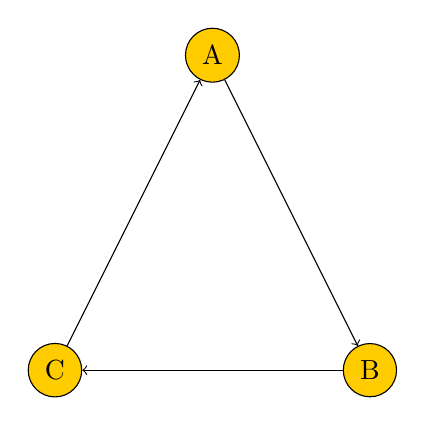
\begin{tikzpicture}[rotate=0,scale=4]
%Define all colors here.

\definecolor{n0fill}{RGB}{255,204,0}
\definecolor{n0text}{RGB}{0,0,0}
\definecolor{n0draw}{RGB}{0,0,0}
\node(A) at (0.5,-0.0) [circle, draw=n0draw, fill=n0fill, text=n0text] {A};

\definecolor{n1fill}{RGB}{255,204,0}
\definecolor{n1text}{RGB}{0,0,0}
\definecolor{n1draw}{RGB}{0,0,0}
\node(C) at (0.0,-1.0) [circle, draw=n1draw, fill=n1fill, text=n1text] {C};

\definecolor{n2fill}{RGB}{255,204,0}
\definecolor{n2text}{RGB}{0,0,0}
\definecolor{n2draw}{RGB}{0,0,0}
\node(B) at (1.0,-1.0) [circle, draw=n2draw, fill=n2fill, text=n2text] {B};

\draw[->] (A) edge (B);
\draw[->] (B) edge (C);
\draw[->] (C) edge (A);
\end{tikzpicture}
